\subsection{规范描述符与比较规则}

容器将每种处理方案转换为一个独立于其源语法的 JSON 描述符。该描述符
记录运行控制参数、块、工具箱、初始工作区、生成器和加载错误。每个块会进一步
分解为原子属性：输入顺序、字段、类型检查、连接、布局、颜色、帮助提示文本、
帮助链接和动态行为。JSON 属性的排列顺序无关紧要，但字段、输入、类别及
工具箱元素的可见顺序会被保留。

每个观测到的属性都会被赋予以下状态之一：

\begin{itemize}
  \item \texttt{match}：值和可观测行为等价；
  \item \texttt{partial}：对同一能力的近似实现，但存在一项有明确记录的具体差异；
  \item \texttt{mismatch}：该能力存在，但生成的值不一致；
  \item \texttt{unsupported}：当前生成链中不存在相应表示；
  \item \texttt{error}：生成的块或编辑器无法加载；
  \item \texttt{excluded}：观测到的差异属于已排除的执行层，不计入分母。
\end{itemize}

每项初步判定为有差异的属性都必须对应唯一一条评估规则，由该规则说明相关能力、
涉及的局限及理由。如果某项差异没有对应规则、同一属性适用两条规则，或某条
规则已不再与结果相符，验证都会失败。这一条件可以防止为了提高最终数值而悄然
重新归类某项差异。

RQ1（功能复现）的主要指标为：

\begin{equation}
  \text{编辑器一致率} =
  \frac{\text{状态为 \texttt{match} 的属性}}
       {\text{可适用属性}} \times 100.
  \label{eq:paridad-editor}
\end{equation}

分母包括 \texttt{match}、\texttt{partial}、\texttt{mismatch}、
\texttt{unsupported} 和 \texttt{error}。\texttt{excluded} 差异会单独
报告。某案例在无错误且达到 100\,\% 时归类为\emph{完整}；能够加载但仍
存在差异时归类为\emph{部分复现}；编辑器或其主要块无法加载时则归类为
\emph{不可复现}。生成器采用相同的状态，但其一致率不计入编辑器的主要得分，
而是另行报告。

\subsection{规格编写工作量指标}

RQ2（规格编写工作量）比较的是需要维护的源文件，而非生成的输出。在 BASELINE
中，只统计该配置所需的定义、编辑器扩展、工具箱构造和生成器。许可证、导入、
容器 HTML、翻译、领域引擎和程序库均排除在外。在 M2B 中统计
\texttt{source.m2b} 文件；生成的 JavaScript 和 HTML 不纳入度量。

对于两种处理方案，都会记录 UTF-8 字节数、总行数、非空行数以及不含注释的
非空行数。主要比较采用最后一种单位：

\begin{equation}
  \text{LOC 缩减率} =
  \left(1 - \frac{\text{LOC}_{\mathrm{m2b}}}
                    {\text{LOC}_{\text{官方}}}\right) \times 100.
  \label{eq:reduccion-loc}
\end{equation}

本文给出各案例的数值、均值、中位数和加权总计。Pond Tutor 和 Pond 复用了
相同官方文件中的若干行。因此，除了将十种配置作为独立产物相加之外，还会计算
一个保守总计，并逐行去重：仅当仓库、修订版本、路径和行号全部相同时，才将该行
官方代码视为重复。十个 \texttt{.m2b} 模型仍保留在该计算中，因为它们是作为独立规格
分别维护的。

Ecore 被有意排除在这一指标之外。将 XML/XMI 的 LOC 与 DSL 的 LOC 比较，
会混合不同的编辑单位。在 RQ4（输入路线）中，Ecore 与 \texttt{.m2b} 的
描述符必须在运行控制参数、块、工具箱、初始工作区、生成器、错误和可加载性方面严格
相同；结果只有等价或不等价两种，并同时给出可能存在的差异。

\section{评估流程与可复现性}
\label{sec:procedimiento-evaluacion-blockly}

每个案例均遵循同一流程：

\begin{enumerate}
  \item 锁定仓库、修订版本和具体配置；
  \item 确定纳入范围的官方代码片段；
  \item 在不作修改的情况下将其提取出来，并核验行号区间和哈希；
  \item 编写该编辑器的 \texttt{.m2b} 模型；
  \item 执行实际生成链；
  \item 在相同的浏览器受控环境下加载 BASELINE 和 M2B；
  \item 实例化各个块并取得规范描述符；
  \item 比较描述符属性，并要求每项差异都有唯一的理由；
  \item 使用同一个度量程序收集 LOC 和字节数；
  \item 保存 JSON 结果和截图，作为可复现证据。
\end{enumerate}

截图可用于检查各处理方案能否正常加载并呈现预期的块，但不作为像素级等价的
证据。判定依据是结构属性和浏览器观测到的错误。对于 E01、E03 和 E07，随后
还会增加 Ecore 生成，并要求其描述符与 M2B 描述符完全相同。

语料集、控制变量和修订版本均在清单
\path{evaluation/official-blockly/}\allowbreak\path{manifest.json} 中声明。
每个案例目录包含官方代码提取结果、\path{source.m2b}、生成输出、评估规则、
描述符、指标和截图。命令 \texttt{npm run\allowbreak{} verify:\allowbreak{}evaluation-\allowbreak{}completed}
会运行容器和全部十个案例；\texttt{npm run\allowbreak{} aggregate:\allowbreak{}evaluation} 会重新生成
全局汇总。保留各案例的单独结果，既可以防止均值掩盖个别案例，也可以将每项
局限追溯到具体属性。

前两个案例 Graph 和 Maze 被用作试点，以便在完成整个语料集之前确定描述符模式、
字段匹配方式和比较状态。标准确定后，便以相同粒度应用于其余八个案例。下一节将
介绍使用这一协议得到的结果。

\section{功能复现结果}
\label{sec:resultados-reproduccion}

表~\ref{tab:resultados-casos-blockly} 汇总了各案例的结果。“编辑器”列衡量
块和工具箱的结构属性；“生成器”列衡量纳入范围的生成属性。两列都以“匹配数/
可适用属性数”的形式显示。范围之外的差异不计入分母。最后三列比较官方配置的
LOC 与 \texttt{.m2b} 模型的 LOC。

\begin{table}[htbp]
  \centering
  \caption{各案例结果：功能一致率与规格编写工作量}
  \label{tab:resultados-casos-blockly}
  \resizebox{\textwidth}{!}{%
  \begin{tabular}{llrrrrrrrr}
    \toprule
    案例 & 编辑器 & 块数 & 编辑器 $m/a$ & 编辑器（\%） & 生成器 $m/a$ & 生成器（\%） & 官方 LOC & M2B LOC & 缩减率（\%） \\
    \midrule
    E01 & Graph       &  2 &  77/91  & 84,62 &  7/8   & 87,50 & 329 &  28 & 91,49 \\
    E02 & Wait        &  1 &  73/89  & 82,02 &  4/4   & 100,00 & 282 &  16 & 94,33 \\
    E03 & Maze        &  5 & 111/137 & 81,02 & 15/15  & 100,00 & 178 &  73 & 58,99 \\
    E04 & Bird        &  8 & 203/218 & 93,12 & 27/31  & 87,10 & 246 &  93 & 62,20 \\
    E05 & Movie       &  5 & 236/283 & 83,39 & 16/20  & 80,00 & 449 &  75 & 83,30 \\
    E06 & Music       &  6 & 186/232 & 80,17 & 19/21  & 90,48 & 545 &  94 & 82,75 \\
    E07 & Turtle      & 12 & 349/427 & 81,73 & 30/40  & 75,00 & 669 & 190 & 71,60 \\
    E08 & Puzzle      &  3 &  59/75  & 78,67 &  6/12  & 50,00 & 221 &  46 & 79,19 \\
    E09 & Pond Tutor  & 11 & 340/397 & 85,64 & 35/44  & 79,55 & 415 & 154 & 62,89 \\
    E10 & Pond        & 24 & 681/813 & 83,76 & 68/96  & 70,83 & 740 & 352 & 52,43 \\
    \midrule
    总计 & & 77 & 2315/2762 & 83,82 & 227/291 & 78,01 & 4074 & 1121 & 72,48 \\
    \bottomrule
  \end{tabular}%
  }
\end{table}

编辑器共有 2762 项可适用属性，其中 2315 项匹配，对应的加权一致率为
83,82\,\%。各案例未加权均值为 83,41\,\%，中位数为 82,71\,\%。其范围
从 Puzzle 的 78,67\,\% 到 Bird 的 93,12\,\%。20 个 BASELINE/M2B
处理实例均无错误加载，模型声明的所有块都能成功实例化。不过，十个案例中没有
任何一个达到 100\,\%：它们都被归类为\emph{部分复现}，而非完全等价。

表~\ref{tab:estados-agregados} 所示的状态汇总分布揭示了单一分数会掩盖的
信息。具体而言，编辑器的 366 项属性和生成器的 50 项属性目前仍无法通过通用
规格表达。编辑器的八项 \texttt{mismatch} 对应于对保留块的重新定义；
生成器的六项则集中在 Puzzle 的自动序列化上。

\begin{table}[htbp]
  \centering
  \caption{比较状态的汇总分布}
  \label{tab:estados-agregados}
  \begin{tabular}{lrr}
    \toprule
    状态 & 编辑器 & 生成器 \\
    \midrule
    \texttt{match}       & 2315 & 227 \\
    \texttt{partial}     &   73 &   8 \\
    \texttt{mismatch}    &    8 &   6 \\
    \texttt{unsupported} &  366 &  50 \\
    \texttt{error}       &    0 &   0 \\
    \texttt{excluded}    &    0 &  17 \\
    \bottomrule
  \end{tabular}
\end{table}

图~\ref{fig:evidencia-visual-corpus} 展示了两组有代表性的对比：复杂度中等的
Maze，以及语料集中规模最大的 Pond。截图证实，两种处理方案都能加载可比较的
工具箱和工作区。不过，截图无法取代结构比较：两幅视觉上相近的截图仍可能掩盖
连接、字段内部值或生成器方面的差异。

\begin{figure}[p]
  \centering
  \begin{minipage}{0.48\textwidth}
    \centering
    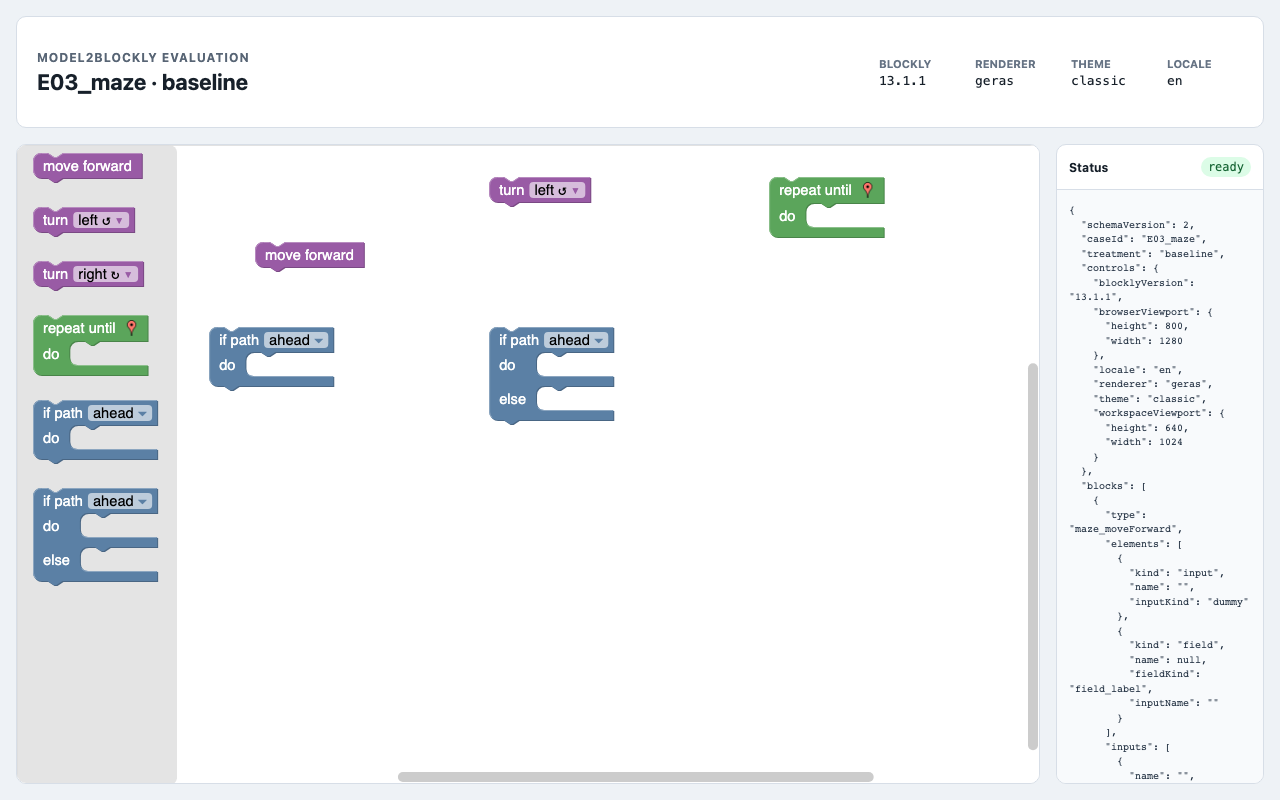
\includegraphics[width=\linewidth]{../../evaluation/official-blockly/cases/E03_maze/results/screenshots/baseline.png}
    \\[2pt]\small (a) 官方 Maze
  \end{minipage}\hfill
  \begin{minipage}{0.48\textwidth}
    \centering
    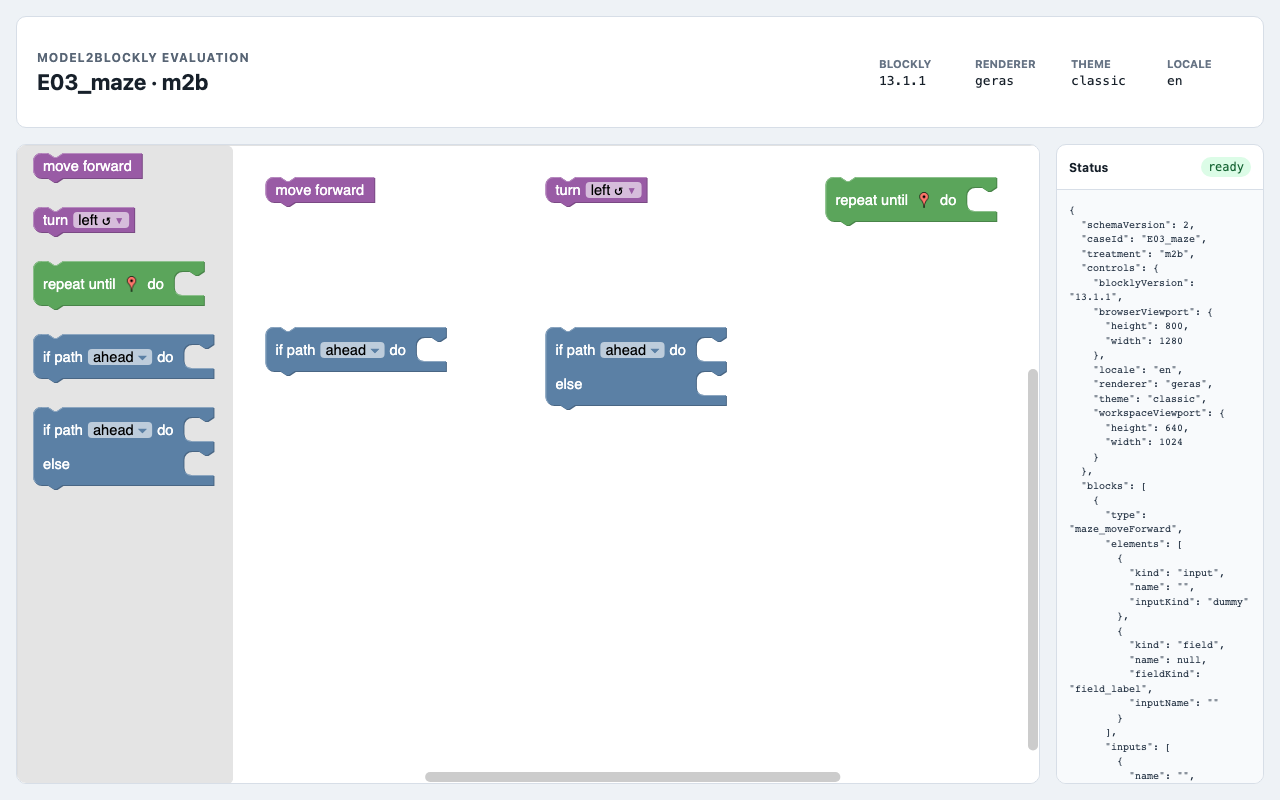
\includegraphics[width=\linewidth]{../../evaluation/official-blockly/cases/E03_maze/results/screenshots/m2b.png}
    \\[2pt]\small (b) 由 M2B 生成的 Maze
  \end{minipage}

  \vspace{0.8em}

  \begin{minipage}{0.48\textwidth}
    \centering
    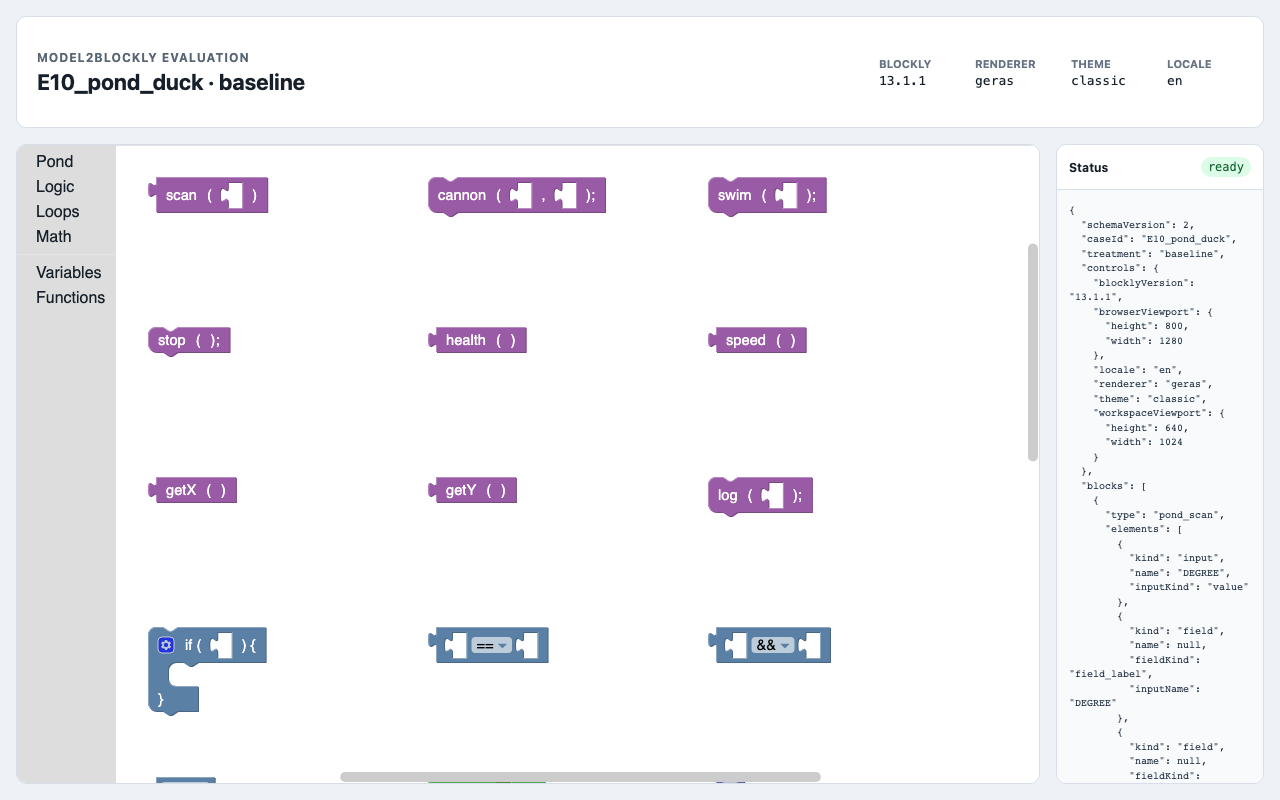
\includegraphics[width=\linewidth]{../../evaluation/official-blockly/cases/E10_pond_duck/results/screenshots/baseline.png}
    \\[2pt]\small (c) 官方 Pond
  \end{minipage}\hfill
  \begin{minipage}{0.48\textwidth}
    \centering
    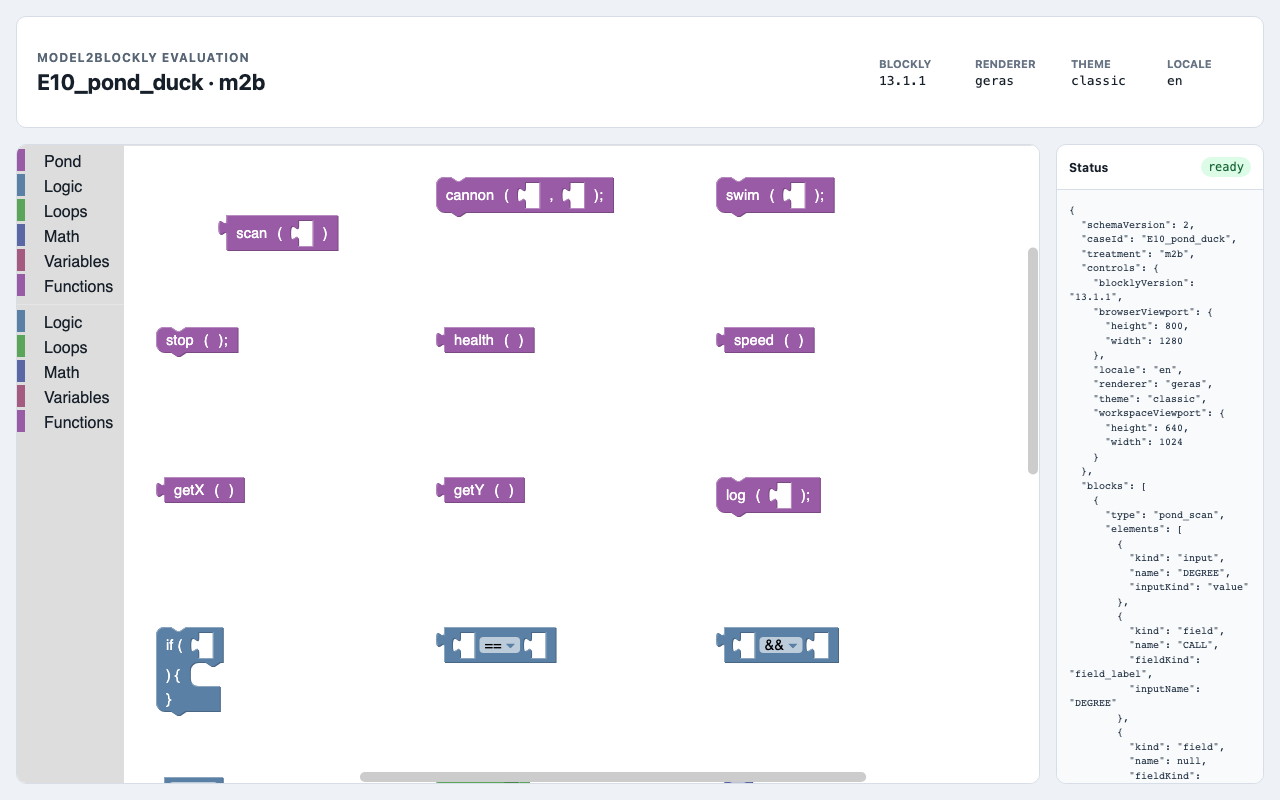
\includegraphics[width=\linewidth]{../../evaluation/official-blockly/cases/E10_pond_duck/results/screenshots/m2b.png}
    \\[2pt]\small (d) 由 M2B 生成的 Pond
  \end{minipage}
  \caption{语料集中两个案例的辅助视觉证据}
  \label{fig:evidencia-visual-corpus}
\end{figure}

\subsection{生成器结果}

生成器的加权一致率为 227/291，即 78,01\,\%。各案例均值为 82,05\,\%，
中位数为 83,55\,\%。有十七项属性标记为 \texttt{excluded}：它们属于
Blockly Games 的执行跟踪和循环中断机制，这些机制会对面向教育应用的程序
进行插桩，但既不定义编辑器，也不定义每种块的基础转换。

Wait 和 Maze 的结果在纳入范围内达到 100\,\%，而 Puzzle 为 50\,\%。
后者得分较低的主要原因是，官方案例会自动序列化整个拼图的状态，而
Model2Blockly 生成的是与块类型关联的函数。此外，Pond 案例中还包含过程、
变量和变形器，它们要求生成期间存在共享状态。因此，这一层得分较低并不意味着
编辑器无法加载，而是说明当前契约并不总能重构官方的生成语义。
